%%%%%%%%%%%%%%%%%%%%%%%%%%%%%%%%%%%%%%%%%%%%%%%%%%%%%%%%%%%%%%%%%
\subsubsection{Theorem 5}		%	TESTFÄLLE - RMin
%%%%%%%%%%%%%%%%%%%%%%%%%%%%%%%%%%%%%%%%%%%%%%%%%%%%%%%%%%%%%%%%%

\noindent
Nach Theorem~\ref{theo: min_5} benötigt \Rm $\mathbb{E}[\mfgm]=\mathcal{O}(\varepsilon^{-1}\log\log(n))$ Vergleiche für das Minimum und $\mathbb{E}[\mfgr]=\mathcal{O}(n^{\varepsilon})$ für alle übrigen Elemente.\\[.1cm]
Da $k(n)$ bei der Eingabe ganzzahlig sein muss, wurde der Wert vor der Eingabe sowohl auf- als auch abgerundet und beide Fälle separat betrachtet. Wie zuvor wird für beide Fälle einen passenden Fit $F_{\lceil k \rceil}(n)$ beziehungsweise $F_{\lfloor k \rfloor}(n)$ untersucht. Für eine präzisere Repräsentation des Parameters $k(n)$ wird zusätzlich ein weiter Fit mit folgender Gewichtung gebildet:
\[F^{\star}(n) = (\lceil k \rceil - k) \cdot f_{\lfloor k\rfloor}(n) + (k - \lfloor k \rfloor)\cdot f_{\lceil k \rceil}(n)
\]\label{other: weigh}

\noindent
Hierbei werden die auf- und abgerundeten Werte relativ entsprechend ihrer absoluten Differenz von dem realen Wert des Parameters $k(n)$ gewichtet. Die Repräsentation für Theorem~\ref{theo: min_5} beruht auf Eingaben für $\log_2(n)=\{6,\cdots,20\}$, mit denen wie zuvor zuerst die \fg des Minimums \fgm und dann die aller übrigen Elemente \fgr experimentell analysiert werden.

%%%%%%%%%%%%%%%%%%%%%%%%%%%%%%%%%%%%%%%%%%%%%%%%%%%%%%%%%%%%%%%%%
%	FRAGILE COMPLEXITY - MINIMUM
\subsubsection*{\textit{Fragile complexity} des Minimum Elements}
Nun wird die Aussage von Theorem~\ref{theo: min_5} bezüglich der \fg des Minimums \fgm untersucht. Es wurden nun wie besprochen drei separate Fits bezüglich der entsprechend gesammelten Datenmenge gebildet. Bei einer Wahl der Startwerte von $a=5$, $b=0.001$ ist der Fit nach $8$, für $a=6.5$, $b=-8.5$ nach $4$ Iteration konvergiert und es ergab sich in beiden Fällen:
\begin{center}
\begin{tabular}{c||l|l|l|l}

&\multicolumn{1}{c|}{Param $a$}&
\multicolumn{1}{c|}{Param $b$}&
\multicolumn{1}{c|}{Sum Res}&
\multicolumn{1}{c}{$\Delta$ Last Iter}\\
\hline
$F_{\lceil k \rceil}(n)$:&$6.97$&$-9.91$&$0.4546$&$-3.23746e-09$\\
\hline
$F_{\lfloor k \rfloor}(n)$:&$6.42$&$-7.88$&$2.2034$&$-4.2210e-13$\\
\hline
$F^{\star}(n)$:&$6.66$&$-8.78$&$1.3096$&$-8.8166e-10$
\end{tabular}
\end{center}

\noindent
Wie zu erkennen, ist die sich ergebende Parametrisierung von $a$ und $b$ in allen Fällen relativ ähnlich. Die Parameter fallen für $F_{\lfloor k \rfloor}(n)$ am geringsten aus, jedoch ist die Summe der Residuenquadrate hier auch am Höchsten.\\[.1cm]
Wie in Abbildung~\ref{fig: min_theo5_fit_min} zu sehen, weicht die gesammelte Datenmenge vorerst leicht von der Prognose des Theorems ab. Skaliert man diese jedoch entsprechend des errechneten Fits, so ergibt sich eine beinahe deckungsgleiche Darstellung zu der gesammelten Datenmenge. Der Fit ist so eindeutig, dass auf eine einfach-logarithmische Abschätzung als Vergleich verzichtet wurde.

% ---------------------------------------------------------------
%	FIG: FG Min
\begin{figure}[H]
	\hspace*{-.4cm}
    \begin{minipage}[t]{.30\textwidth}
        \centering
        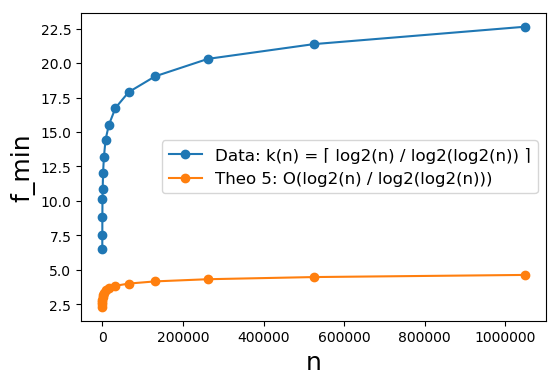
\includegraphics[width=1.1\textwidth]{pictures/min_theo5_min_ceil_pred.png}
        \vspace*{-0.06cm}
    \end{minipage}
    \hspace*{.4cm}
    \begin{minipage}[t]{.30\textwidth}
        \centering
        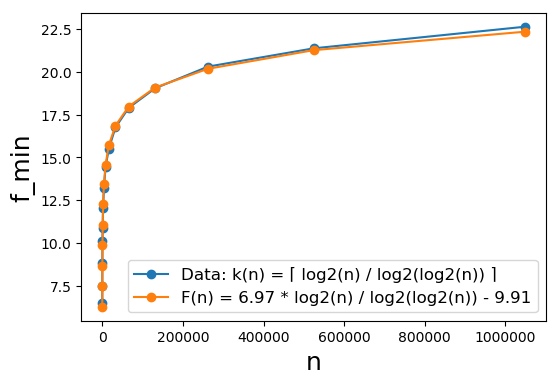
\includegraphics[width=1.11\textwidth]{pictures/min_theo5_min_ceil_fit.png}
    \end{minipage}
    \hspace*{.4cm}
    \begin{minipage}[t]{.30\textwidth}
        \centering
        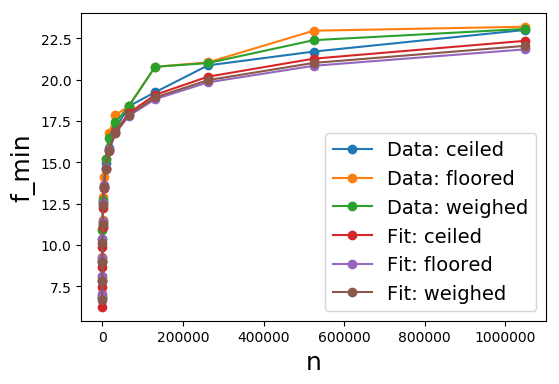
\includegraphics[width=1.11\textwidth]{pictures/min_theo5_min_all.png}
    \end{minipage}
    \vspace*{-0.1cm}
    \captionof{figure}{Vorhersage und Fit für \fgm bezüglich Auf- und Abrundung.}\label{fig: min_theo5_fit_min}
\end{figure}

% ---------------------------------------------------------------
\noindent
Dies lässt die Aussage von Theorem~\ref{theo: min_5} bezüglich der \fg des Minimums \fgm eindeutig bestätigen.

\subsubsection*{\textit{Fragile complexity} aller nicht-Minimum Elemente}
Nun wird eine analoge Betrachtung bezüglich der \fg aller übrigen Elemente $f_{rem}(n)$ durchgeführt. Die Prognose von Theorem~\ref{theo: min_5} bezüglich der \fg ist identisch für das Minimum und für alle übrigen Elemente. Das Ergebnis für \fgr weist keine Unregelmäßigkeiten auf und es bilden sich ähnliche Abschätzungen wie bereits für $f_{min}(n)$:

\begin{center}
\begin{tabular}{c||l|l|l|l}

&\multicolumn{1}{c|}{Param $a$}&
\multicolumn{1}{c|}{Param $b$}&
\multicolumn{1}{c|}{Sum Res}&
\multicolumn{1}{c}{$\Delta$ Last Iter}\\
\hline
$F_{\lceil k \rceil}(n)$:&$7.14$&$-10.38$&$0.8468$&$-7.22016e-09$\\
\hline
$F_{\lfloor k \rfloor}(n)$:&$7.44$&$-10.96$&$2.0026$&$-8.9850e-10$\\
\hline
$F^{\star}(n)$:&$7.37$&$-10.88$&$1.8968$&$-9.3543e-10$
\end{tabular}
\end{center}

\noindent
Abschließend sei hier noch anzumerken, dass die für diese Eingabe von \Rm benötigte Arbeit $w(n)$ mit wachsendem $n$ linear skaliert. Somit kann die Aussage von Theorem~\ref{theo: min_3} weiterhin bestärkt werden und neben einer Darstellung des Fits für \fgr abschließend in Abbildung~\ref{fig: min_theo5_fit_rem} eingesehen werden. 

% ---------------------------------------------------------------
%	FIG: FG Min
\begin{figure}[H]
	\hspace*{-1.1cm}
    \begin{minipage}[t]{.30\textwidth}
        \centering
        \raisebox{0.05cm}{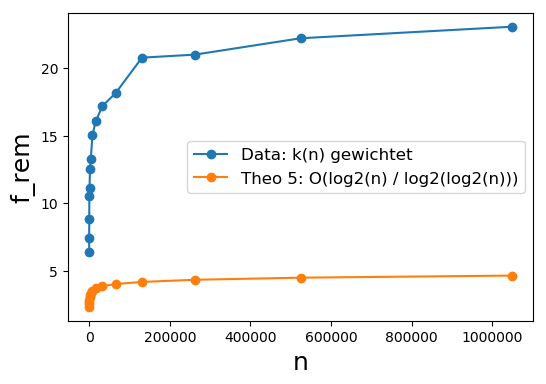
\includegraphics[width=1.15\textwidth]{pictures/min_theo5_rem_weigh_pred.png}}
    \end{minipage}
    \hspace*{.6cm}
    \begin{minipage}[t]{.30\textwidth}
        \centering
        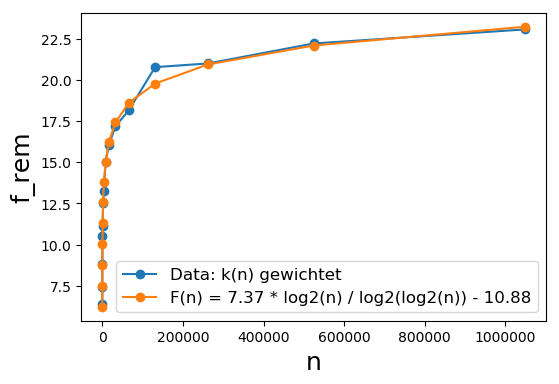
\includegraphics[width=1.2\textwidth]{pictures/min_theo5_rem_weigh_fit.png}
    \end{minipage}
    \hspace*{.8cm}
    \begin{minipage}[t]{.30\textwidth}
        \centering
        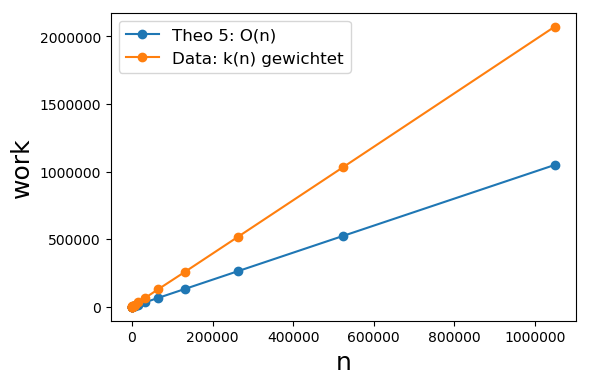
\includegraphics[width=1.25\textwidth]{pictures/min_theo5_work_weigh_pred.png}
    \end{minipage}
    \vspace*{-0.1cm}
    \captionof{figure}{Vorhersage und Fit für \fgr sowie die Arbeit $w(n)$.}\label{fig: min_theo5_fit_rem}
\end{figure}

% ---------------------------------------------------------------
\noindent
Dies beendet die experimentelle Analyse dieser Arbeit bezüglich des in Paper~\cite{meyer1} vorgestellten Algorithmus \Rm und der \fg des Minimums sowie aller übrigen Elemente.\\[.1cm]
Es konnte ein Zusammenhang zwischen den Eingabeparametern $n$ und $k(n)$ sowie der Güte der Filterung der ersten drei Phasen nachgewiesen, sowie die Aussagen der Theoreme 3-5 des Papers eindeutig bekräftigt werden.\\[.1cm]
Weitere untersuchte Fälle liegen der Arbeit bei und können zusätzlich im Anhang nachgeschlagen werden. 

%%%%%%%%%%%%%%%%%%%%%%%%%%%%%%%%%%%%%%%%%%%%%%%%%%%%%%%%%%%%%%%%%